\subsection{Bestehende Konzepte und zukünftige Flugzeugmodelle}
In diesem Teil ist beschrieben, welche Flugzeugmodelle und -konfigurationen 
mit im Teil \ref{s:Neuartige Antriebe} beschriebenen Antrieben in näherer Zukunft zu erwarten sind. 
Vor allem sind hier die Modelle ohne hybride Nutzung fossiler Energieträger zusammengefasst.

Aufgrund ihrer Drop-In Fähigkeit werden die SAFs keine neuen Luftfahrzeugkonfigurationen brauchen. 
Was als Vorteil für den SAF betrachtet werden kann, 
angesichts der aktuell produzierten Flugzeuge welche
mindestens 20 Jahre im Einsatz sein werden \cite{austr}.  
%Die Abbildung stellt Eintrittsjahre für alternative Antriebe dar. %%%%%%%%%%%%%%%%%%%%%%        BILD?
Kleinere Flugzeuge mit elektrischem Antrieb sind bereits jetzt im Einsatz zu finden. 
Mit weiterer Entwicklung des Batterieantriebs bis Jahr 2030 zu rechnen \cite{austr}.  %%% versuche morgen zu umformulieren
Der Betrieb der Brennstoffzelle mit Wasserstoff ist zwischen 2030 und 2040 zu erwarten, 
wobei Wasserstoffturbinen werden frühestens ab 2040 eingesetzt \cite{austr}. 

%
Positive Auswirkungen auf Emissions-Werte können bereits mit bestimmten 
Flugzeug- und Triebwerkskonfigurationen erreicht werden.
Zum Beispiel \textit{Claire Liner} vom Bauhaus Luftfahrt e. V. München 
bringt nicht nur aerodynamische Vorteile mit, sondern auch eine Verringerung 
des Kraftstoffverbrauchs und damit die Reduktion der Emissionen.
Jedoch sind mehr Änderungen notwendig, um Netto null \ce{CO2}-Werte zu erreichen.
Die Herstellung bereitet Schwierigkeiten, manche Firmen müssen den Geschäftsbetrieb einstellen, 
wie Universal Hydrogen oder Zunum Aero, oder Konzepte werden nicht weiterentwickelt.

Es wurden eine Vielzahl an elektrischen Flugzeugen mit geringer 
Sitzkapazität vorgestellt, einige davon wurden sogar geflogen.
Das Institut für Flugzeugbau der Universität Stuttgart entwickelte 
ein zweisitziges hybrid-batteriebetriebenes Segelflugzeug \textit{e-Genius}. 
Das Flugzeug soll eine Reichweite von 400 km erreichen und hat eine 
Batteriekapazität von 40 kWh mit 1,5 Stunden Ladedauer \cite{IFB_eGenius_2025}.
Pipistrel Alpha Electro hat bereits im Jahr 2007 seinen ersten elektrischen Zweisitzer vorgestellt, 
mittlerweile wird das Modell \glqq Velis Electro\grqq{} \cite{Pipistrel_VelisElectro} für 
das Pilottraining mit einem Triebwerk mit 57.6 kW Leistung genutzt. 
Der Antrieb ist flüssigkeitsgekühlt und braucht ein externes Ladegerät. 
Das neunsitzige vollelektrische Flugzeug \textit{Alice} von Eviation, 
mit 250 NM Reichweite und jeweils zwei Triebwerken von 700 kW Leistung,
macht bereits Fortschritte in Zertifizierungsrichtung.
%
Die größeren Konzepte hingegen haben aufgrund der Komplexität der Technologien 
und Gewicht mit der Umsetzung zu kämpfen.\\
%\begin{figure}[h]
%	\centering
%	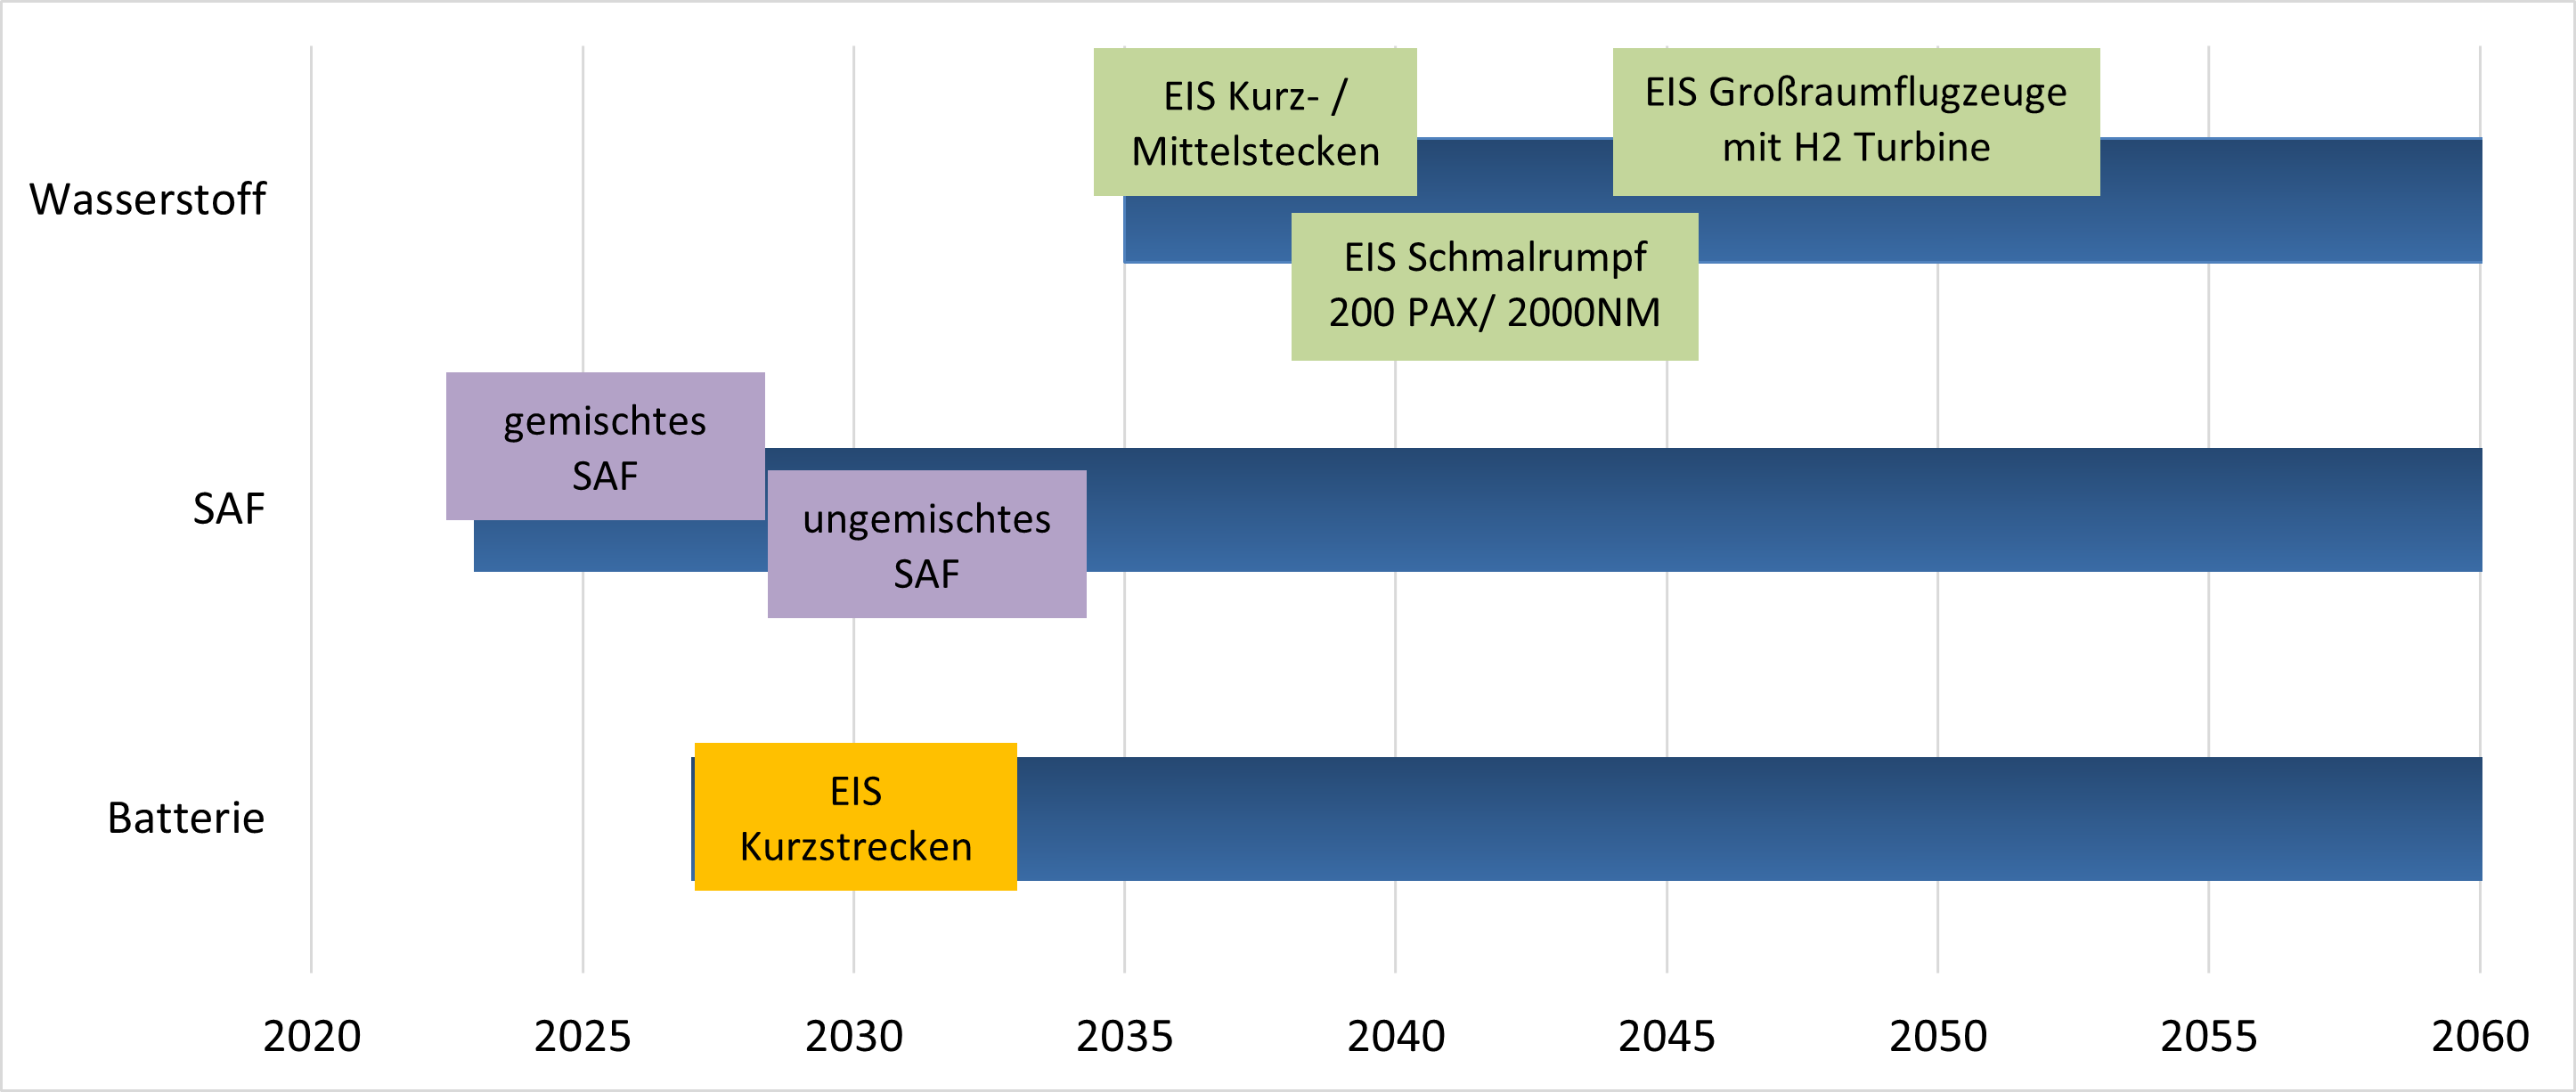
\includegraphics[width=0.7\linewidth]{Bilder/eis.png}
%	\caption[Eintrittsjahren ]{ wird ausgetauscht durch tatsächlichen EIS}
%	\label{eis_konzepte}
%\end{figure}

\subsubsection{Konfigurationen mit Batterieantrieb}

Wie bereits erwähnt wurde, haben die zurzeit bestehenden Batterien die geringe Energiedichte. 
Deshalb ist zu erwarten, dass bis zum Jahr 2050 keine großen vollelektrischen Flugzeuge hergestellt werden \cite{mukhopadhaya2022performance}, 
stattdessen werden die Regional- und Kurzstrecken in den Mittelpunkt gestellt.

Ein vielversprechender Prototyp war die \textit{ES-19} von Heart Aerospace. 
Das Unternehmen versprach die Beförderung von 19 Passagieren über 400 km mit einem BA. 
Das Flugzeug war für Regionalstrecken konzipiert und 
somit konnte die geringe Nachfrage gedeckt werden. 
Außerdem wurden geringe Betriebs- und Wartungskosten erwartet \cite{dalmia2022powering}.
Die ES-19 wurde auf das aktuellste Modell, die ES-30, 
mit einen hybriden Wasserstoffantrieb umgerüstet.

Eines der größten Konzepte mit vollelektrischen Abtrieb stellte Bauhaus Luftfahrt vor. 
Das Passagierflugzeug \textit{Ce-Liner} \cite{BauhausLuftfahrt} ist mit einer 
C-Wing-Konfiguration\footnote{C-Wing-Konfiguration bezeichnet ein Flugzeugdesign, bei dem Tragflächen und integrierte Winglets in einer C-Form angeordnet sind}
ausgestattet und sollte eine Reichweite von 900 NM haben und 190 Passagiere befördern. 
Die benötigte Batteriekapazität wurde auf 2000 Wh/kg eingeschätzt. 
Die Batteriemodule sollen bei Turnaround ausgewechselt werden.

\subsubsection{Konfigurationen mit Wasserstoffantrieb}

Embraer zeigte eine Reihe von nachhaltigen Flugzeugen \textit{ENERGIA}. 
Die Flugzeuge sind mit unterschiedlichen Antrieben ausgestattet, 
unter anderem hybrid-elektrisch oder mit Brennstoffzelle und Wasserstoffturbine. 
Bei der Wasserstoffturbine wurde das Konzept von Dualem-Treibstoff vorgeschlagen, 
bei welchem entweder Jet-A/SAF oder Wasserstoff genutzt werden kann. 
Das Unternehmen spricht von einer Technologiebereitschaft ab dem Jahr 2030, 
für die Wasserstoffturbine ab dem Jahr 2035 und der Wasserstoffturbine ab dem Jahr 2040 \cite{embraer_energia_2021}. % MAX: hier wiederholst du dich oder?
%
Airbus \cite{airbus_zea_concepts} hat im Jahr 2020 drei unterschiedliche 
emissionsfreie \textit{ZEROe} Konzepte vorgestellt: Turbofan, Turboprop und eins mit „Blended-wing body“-Design.
In allen Konzepten ist Wasserstoff und ein Antrieb mit Gasturbinentriebwerk im Einsatz. 
Die Reichweite bewegt sich in einem Bereich von über 1850 - 3700 km 
und die Anzahl beförderter Passagiere wird von auf 100 bis 200 geschätzt. 
Das Unternehmen will die Technologien bis zum 2035 zur Einsatzreife bringen.

Wright Spirit \cite{wright_electric_website} hat ein Konzept auf Basis 
des konventionellen Flugzeugs BAe 146 vorgestellt, allerdings mit einem Wasserstoffantrieb.
Das Flugzeug soll mit vier Triebwerken, 2,5 MW Motoren und vorgestellter Batterie 
mit 800 Wh/kg eine Reichweite von 1000 km erreichen und 100 Passagiere transportieren.

NASA hat das turboelektrische, mit flüssigen Wasserstoff angetriebene 
Konzept N3-X \cite{NASA_N3X_2025} vorgeschlagen.
Das Modell ist mit \textit{Blended Wing Body} (Abb. \ref{NASA_konfig}) konzipiert und verspricht, 
dass der Treibstoffverbrauch bis um 70 \% reduziert werden kann.
\begin{figure}[h]
	\centering
	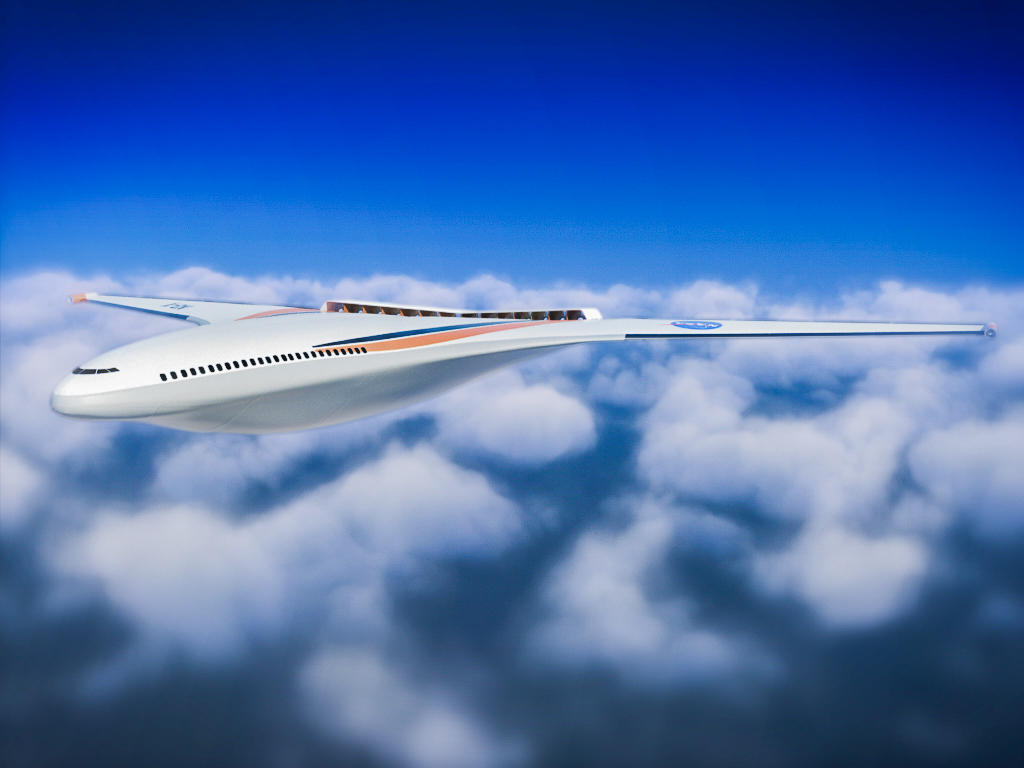
\includegraphics[width=0.6\linewidth]{Bilder/NASA.jpg}
	\caption[Konzeptflugzeug mit Blended Wing Body N3-X]{Konzeptflugzeug mit Blended Wing Body N3-X \cite{NASA_N3X_2025} }
	\label{NASA_konfig}
\end{figure}

ZeroAvia stellt ihre hybrid Wasserstoff-elektrischen Antriebe 
mit drei unterschiedlichen Leistungen und Kapazitäten vor. 
Der kleinste Antrieb, ZA600, hat mit einer Leistung von 600 kW,
die Möglichkeit bis zu 20 Passagiere über 555 km zu befördern. 
Die geplante Eintrittzeit (Entry-in-System - EIS) ist im Jahr 2025. 
Das Luftfahrzeug wird mit gasförmigem Wasserstoff angetrieben.
%Flugzeug mit 80 Menschen verbraucht bis zu 80% weniger Treibstoff pro STD/kg (5 mal weniger)
%
Abschließend lässt sich feststellen, dass aktuell zahlreiche Konzepte ausgearbeitet werden. 
Wie erfolgreich diese sind, ist abzuwarten bis Technologien tatsächlich auf den Markt kommen.
